\section{Lorenz Gauge and gravitational waves}

    Lets remember how are the conditions of thte gravitational field we're working on (there is only one v:) which is a \textit{theory of weak field} this means we have a plane (Minkowski) space-time but there is a certain perturbation on a region we represent it as $g_{\alpha\beta} = \eta_{\alpha\beta} + h_{\alpha\beta}\;|h_{\alpha\beta}| \ll 1 $. We can do these perturbations on the coordinate charts as $x'^{\alpha} =x^{\alpha} + \xi^{\alpha} $ where $\xi^{\alpha}=\xi^{\alpha}(x^{\alpha}) $ are infinitesimal transformations such that

    \begin{equation}
        \left|\frac{\partial \xi^{\alpha}}{\partial x^{\beta}} \right| \approx |h_{\alpha\beta}| \rightarrow \left|\frac{\partial \xi^{\alpha}}{\partial x^{\beta}} \right| \ll 1.
    \end{equation}

    We are looking for a gauge theory that leaves invariant certain quantity, in our case such quantity is the Riemann's tensor, to do it we gotta see how is the behavior of our space-time

    \begin{equation}
        g'_{\alpha\beta}=g_{\mu\nu}\frac{\partial x^{\mu}}{\partial x'^{\alpha}}\frac{\partial x^{\nu}}{\partial x'^{\beta}},
    \end{equation}

    \begin{equation}
        \frac{\partial x^{\mu}}{\partial x'^{\alpha}} = \delta^{\mu}_{\;\alpha} - \frac{\partial \xi^{\mu}}{\partial x^{\nu}}\frac{\partial x^{\nu}}{\partial x'^{\alpha}} = \delta^{\mu}_{\;\alpha}-\frac{\partial \xi^{\mu}}{\partial x^{\nu}}\left(\delta^{\nu}_{\;\alpha}-\frac{\partial \xi^{\nu}}{\partial x^{\rho}}\frac{\partial x^{\rho}}{\partial x'^{\alpha}} \right),
    \end{equation}

    \begin{equation}\label{eq:deMuaPrimaAlpha}
        \frac{\partial x^{\mu}}{\partial x'^{\alpha}} = \delta^{\mu}_{\;\alpha}-\frac{\partial \xi^{\mu}}{\partial x^{\alpha}},
    \end{equation}

    \begin{equation}
        g'_{\alpha\beta} = g_{\mu\nu}\left(\delta_{\alpha}^{\;\mu} - \frac{\partial \xi^{\mu}}{\partial x^{\alpha}} \right)\left(\delta^{\nu}_{\;\beta} - \frac{\partial \xi^{\nu}}{\partial x^{\beta}} \right) = g_{\alpha\beta} - g_{\alpha\nu}\frac{\partial \xi^{\nu}}{\partial x^{\beta}} - g_{\beta\mu}\frac{\partial \xi^{\mu}}{\partial x^{\alpha}},
    \end{equation}

    \begin{equation}
        g'_{\alpha\beta} = \left(\eta_{\alpha\beta} + h_{\alpha\beta} \right) - \eta_{\alpha\nu}\frac{\partial\xi^{\nu}}{\partial x^{\beta}} - \eta_{\beta\mu}\frac{\partial\xi^{\mu}}{\partial x^{\alpha}},
    \end{equation}

    \begin{equation}
        g'_{\alpha\beta} = \eta_{\alpha\beta}+h'_{\alpha\beta}\;\rightarrow; h'_{\alpha\beta} = h_{\alpha\beta} - \eta_{\alpha\nu}\frac{\partial\xi^{\nu}}{\partial x^{\beta}} - \eta_{\beta\mu}\frac{\partial \xi^{\mu}}{\partial x^{\alpha}}.
    \end{equation}

    {\sloppy\textbf{AQUÍ DEBERÍA AGREGAR ALGO SOBRE TEORÍA DE GAUGE EN EL ELECTROMAGNETISMO COMO ANEXO O COMO NO SÉ XD}\par}

    In analogy to see how transforms the Riemann's tensor, lets first calculate the following transform of the tensor $R'^{\alpha\beta}_{\quad\mu\nu}$ this because it will be easier mathematically calculate in this form and in the end using the Minkowski's metic tensor we can lower one index, therefore

    \begin{equation}\label{eq:TransoformandoAndo}
        R'^{\alpha\beta}_{\quad\mu\nu} = \frac{\partial x'^{\alpha}}{\partial x^{\alpha}}\frac{\partial x'^{\beta}}{\partial x^{b}}\frac{\partial x^c}{\partial x'^{\mu}}\frac{\partial x^{d}}{\partial x'^{\nu}}R^{ab}_{\quad cd}
    \end{equation}

    we gotta calculate the derivative of the prime coordinates repect to the non prime , then

    \begin{equation}\label{eq:DePrimaNoPrima}
        \frac{\partial x'^{\alpha}}{\partial x^{\mu}} = \delta_{\mu}^{\;\alpha} + \frac{\partial \xi^{\alpha}}{\partial x^{\mu}}.
    \end{equation}

    Using the equation \ref{eq:deMuaPrimaAlpha} and \ref{eq:DePrimaNoPrima} into the equation \ref{eq:TransoformandoAndo} we then have

    \begin{align*}
        R'^{\alpha\beta}_{\quad\mu\nu} = \left[\delta_a^{\;\alpha}+\frac{\partial \xi^{\alpha}}{\partial x^a} \right]\left[\delta_b^{\;\beta}+\frac{\partial \xi^{\beta}}{\partial x^b} \right]\left[\delta_{\mu}^{\;c}-\frac{\partial \xi^{c}}{\partial x^{\mu}} \right]\left[\delta_{\nu}^{\;d}-\frac{\partial \xi^{d}}{\partial x^{\nu}} \right]R^{ab}_{\quad cd}\\
        = \left[\delta_a^{\;\alpha}\delta_b^{\;\beta} + \delta_a^{\;\alpha}\frac{\partial \xi^{\beta}}{\partial x^b} + \delta_b^{\;\beta}\frac{\partial\xi^{\alpha}}{\partial x^a} \right]\left[\delta_{\mu}^{\;c}\delta_{\nu}^{\;d} - \delta_{\mu}^{\;c}\frac{\partial\xi^{d}}{\partial x^{\nu}} - \delta_{\nu}^{\;d}\frac{\partial\xi^c}{\partial x^{\mu}} \right]R^{ab}_{\quad cd}\\
        = \left[\delta_a^{\;\alpha}\delta_b^{\;\beta}\delta_{\mu}^{\;c}\delta_{\nu}^{\;d} - \delta_a^{\;\alpha}\delta_b^{\;\beta}\delta_{\mu}^{\;c}\frac{\partial\xi^d}{\partial x^{\nu}} - \delta_a^{\;\alpha}\delta_b^{\;\beta}\delta_{\nu}^{\;d}\frac{\partial \xi^c}{\partial x^{\mu}} + \delta_a^{\;\alpha}\delta{\mu}^{\;c}\delta_{\nu}^{\;d}\frac{\partial x^{\beta}}{\partial x^b} + \delta_b^{\;\beta}\delta_{\mu}^{\;c}\delta_{\nu}^{\;d}\frac{\partial\xi^{\alpha}}{\partial x^a} \right]R^{ab}_{\quad cd}\\
        = R^{\alpha\beta}_{\quad\mu\nu}+\left\{\delta_b^{\;\beta}\delta_{\mu}^{\;c}\left[\delta_{\nu}^{\;d}\frac{\partial\xi^{\alpha}}{\partial x^a} - \delta_a^{\;\alpha}\frac{\partial\xi^d}{\partial x^{\nu}} \right] + \delta_a^{\;\alpha}\delta_{\nu}^{\;d}\left[\delta_{\mu}^{\;c}\frac{\partial \xi^{\beta}}{\partial x^b}-  \delta_b^{\;\beta}\frac{\partial \xi^c}{\partial x^{\mu}} \right] \right\}R^{ab}_{\quad cd}\\
        = R^{\alpha\beta}_{\quad\mu\nu}+\left\{\delta_b^{\;\beta}\delta_{\mu}^{\;c}\left[\delta_{\nu}^{\;d}\delta_{a}^{\;\nu} \frac{\partial\xi^{\alpha}}{\partial x^{\nu}} - \delta_a^{\;\alpha}\delta_{\alpha}^{\;d} \frac{\partial\xi^{\alpha}}{\partial x^{\nu}} \right] + \delta_a^{\;\alpha}\delta_{\nu}^{\;d}\left[\delta_{\mu}^{\;c}\delta^{\mu}_{\;b} \frac{\partial \xi^{\beta}}{\partial x^{\mu}}-  \delta_b^{\;\beta}\delta^c_{\;\beta} \frac{\partial \xi^{\beta}}{\partial x^{\mu}} \right] \right\}R^{ab}_{\quad cd}\\
        = R^{\alpha\beta}_{\quad\mu\nu}+\left\{\delta_b^{\;\beta}\delta_{\mu}^{\;c}\delta^d_{\;a} \left[\frac{\partial\xi^{\alpha}}{\partial x^{\nu}} - \frac{\partial\xi^{\alpha}}{\partial x^{\nu}} \right] + \delta_a^{\;\alpha}\delta_{\nu}^{\;d}\delta^c_{\;b} \left[\frac{\partial \xi^{\beta}}{\partial x^{\mu}}  - \frac{\partial \xi^{\beta}}{\partial x^{\mu}} \right] \right\}R^{ab}_{\quad cd},
    \end{align*}

    \begin{align}
        R'^{\alpha\beta}_{\quad\mu\nu} = R^{\alpha\beta}_{\quad\mu\nu}\\
        \eta_{b\beta} R'^{\alpha\beta}_{\quad\mu\nu} = R'^{\alpha}_{\;b\mu\nu} = \eta_{b\beta} R^{\alpha\beta}_{\quad\mu\nu} = R^{\alpha}_{\;b\mu\nu}  
    \end{align}
    Doing the variable change $b = \beta$ we then arrive that the Riemann's tensor keep invariant under these infinitesimal transformations:

    \begin{equation}
        R'^{\alpha}_{\;\beta\mu\nu} = R^{\alpha}_{\;\beta\mu\nu},
    \end{equation}
    and thus

    \begin{equation}
        R'_{\alpha\beta} = R_{\alpha\beta}
    \end{equation}

    and the Lorenz Gauge is 

    \begin{equation}
        \Vec{\nabla}_{\alpha}\left(\eta^{\alpha\beta}A_{\beta} \right)=0
    \end{equation}

    and then by analogy with the electromagnetism $\overline{h}_{\alpha\beta}$ fulfil a Lorenz Gauge as follows

    \begin{equation}
        \frac{\partial}{\partial x^{\mu}}\left(\eta^{\mu\nu}\overline{h}_{\alpha\nu} \right)=0.
    \end{equation}

    Well then, in the Einstein's equation  \ref{eq:EinsteinEqHbar} there is the trace and the tensors of the trace inverted tensors, so we have to calculate they transformed versions too, in this way lets do it

    \begin{equation}
        h' = h - 2\partial_{\mu}\xi^{\mu},
    \end{equation}

    \begin{equation}
        \overline{h}'_{\alpha\beta} = h'_{\alpha\beta} - \frac{1}{2}\eta_{\alpha\beta}h' = h_{\alpha\beta}-\frac{\partial\xi_{\alpha}}{\partial x^{\beta}} - \frac{\partial \xi_{\beta}}{\partial x^{\alpha}} - \frac{1}{2}\eta_{\alpha\beta}\left(h-2\frac{\partial\xi^{\alpha}}{\partial x^{\mu}} \right),
    \end{equation}

    \begin{equation}
        \overline{h}'_{\alpha\beta}=\overline{h}_{\alpha\beta} - \frac{\partial \xi_{\alpha}}{\partial x^{\beta}} - \frac{\partial \xi_{\beta}}{\partial x^{\alpha}} + \eta_{\alpha\beta}\frac{\partial \xi^{\mu}}{\partial x^{\mu}},
    \end{equation}

    \begin{equation}
        W'_{\alpha} = \frac{\partial}{\partial x^{\mu}}\left(\eta^{\mu\nu}\overline{h}'_{\alpha\nu} \right),
    \end{equation}

    \begin{equation}
        W'_{\alpha}=\partial_{\mu}\left[\eta^{\mu\nu}\left(\overline{h}_{\alpha\nu} - \partial_{\nu}\xi_{\alpha}-\partial_{\alpha}\xi_{\nu}+\eta_{\alpha\nu}\partial_{\mu}\xi^{\mu} \right)\right],
    \end{equation}

    \begin{equation}
        W'_{\alpha} = \partial_{\mu}\left[\eta^{\mu\nu}\overline{h}_{\alpha\nu} - \eta^{\mu\nu}\partial_{\nu}\xi_{\alpha} - \partial_{\alpha}\xi^{\mu} + \delta_{\alpha}^{\;\mu}\partial_{\mu}\xi^{\mu} \right]
    \end{equation}

    \begin{equation}
        W'_{\alpha} = W_{\alpha}-\eta^{\mu\nu}\frac{\partial^2\xi}{\partial x^{\mu}\partial x^{\nu}} \;\rightarrow;W'_{\alpha} = W_{\alpha}-\Box \xi_{\alpha},
    \end{equation}

    \begin{equation}
        W'_{\alpha}=0 \iff W_{\alpha}=\Box\xi_{\alpha}.
    \end{equation}

    We have got a little freedom to choose our $W_{\alpha}$ keeping invariant the Riemann's tensor fulfilling then

    \begin{equation}
        \Box\overline{h}_{\alpha\beta} = -16\pi T_{\alpha\beta},
    \end{equation}

    and turning back the unities therefore

    \begin{equation}\label{eq:GravWaveEq}
        \Box\overline{h}_{\alpha\beta}=-\frac{16\pi G}{C^4}T_{\alpha\beta}.
    \end{equation}

    The equation \ref{eq:GravWaveEq}  is the wave equation for gravitational waves! Lets see how are their solutions, first we are going to analyze the vacuum case $T_{\alpha\beta}=0$ and the simplest  solution would be a traveling monochromatic plane wave as

    \begin{equation}
        \overline{h}_{\alpha\beta}(x^{\mu}) = A_{\alpha\beta}e^{ik_{\mu}x^{\mu}},
    \end{equation}

    using this solution in the equation \ref{eq:GravWaveEq} we find that $k_{\alpha}k^{\alpha}=0$ this means the vector $\mathbb{K}$ is a null-like or light-like vector, this implies that \textit{the gravitational waves travels at the speed of light in vacuum} and from the  Lorenz Gauge we find this

    \begin{equation}
        \frac{\partial}{\partial x^{\mu}}\left(\eta^{\mu\nu}A_{\alpha\nu}e^{ik_{\sigma}x^{\sigma}} \right)=0,
    \end{equation}

    \begin{equation}
        \eta^{\mu\nu}A_{\alpha\nu}\frac{\partial}{\partial x^{\mu}}e^{ik_{\sigma}x^{\sigma}}=0,
    \end{equation}

    \begin{equation}
        \eta^{\mu\nu}A_{\alpha\nu}e^{ik_{\sigma}x^{\sigma}}ik_{\beta}\frac{\partial x^{\beta}}{\partial x^{\mu}} = 0,
    \end{equation}

    \begin{equation}\label{eq:GravWaveOrto}
        \eta^{\mu\nu}A_{\alpha\nu}ik_{\mu}e^{ik_{\sigma}x^{\sigma}}=0.
    \end{equation}

    The equation \ref{eq:GravWaveOrto} means that the wave vector is orthogonal to the amplitude tensor.
\section{Gravitational waves}

    Here we are going to keep developing the wave equation for the perturbation $h_{\alpha\beta}$ see how are the equations for the perturbations of the coordinates components and we will work with a new Gauge, the called \textit{traceless transverse gauge} and we will find out the gravitational waves have got polarization properties. \\

    From our Lorentz gauge we had found that $W'_{\alpha} = 0$ but this also means that the perturbations of the coordinates satisfies a wave equation $W_{\alpha}=\Box \xi_{\alpha}$ so we can suppose the most basic solution to this equation is a plane wave, therefore

    \begin{equation}
        \xi^{\alpha} = B^{\alpha}e^{ik_{\sigma}x^{\sigma}},
    \end{equation}

    where $B^{\alpha}$ are four infinitesimal constants, and we gotta find them to have a complete solution for the wave equation to do it lets start from the primed and bar perturbation

    \begin{equation}
        \overline{h}'_{\alpha\beta} = \overline{h}_{\alpha\beta} - \frac{\partial \xi_{\alpha}}{\partial x^{\beta}} - \frac{\partial \xi_{\beta}}{\partial x^{\alpha}} + \eta_{\alpha\beta  }\frac{\partial \xi_{\mu}}{\partial x^{\mu}},
    \end{equation}

    \begin{equation}
        \overline{h}'_{\alpha\beta} = A_{\alpha\beta}e^{ik_{\sigma}x^{\sigma}} - iB_{\alpha}k_{\beta}e^{ik_{\sigma}x^{\sigma}} - iB_{\beta}k_{\alpha}e^{ik_{\sigma}x^{\sigma}} + i \eta_{\alpha\beta}k_{\sigma}B^{\sigma} e^{ik_{\sigma}x^{\sigma}} = A'_{\alpha\beta}e^{ik_{\sigma}x^{\sigma}},
    \end{equation}
    thus

    \begin{equation}\label{eq:Aprima}
        A'_{\alpha\beta} = A_{\alpha\beta}  - iB_{\alpha}k_{\beta} - i B_{\beta}k_{\alpha} + i \eta_{\alpha\beta}k_{\sigma}B^{\sigma}.
    \end{equation}

    \subsection{Traceless transverse gauge}

        Here we are going to choose a new gauge, the \textit{traceless transverse gauge} which will allow us to work as well with $\overline{h}_{\alpha\beta}$ as $h_{\alpha\beta}$ because, we will see it in a moment, both satisfies the same wave equations. The traceless transerverse Gauge is:

        \begin{equation}
            \eta^{\mu\nu}A'_{\mu\nu}=0,
        \end{equation}

        \begin{equation}
            A'_{oi} = 0.
        \end{equation}

        Calculating the Gauge of the equation \ref{eq:Aprima} we have

        \begin{align}
            \eta^{\mu\nu}A'_{\mu\nu} = \eta^{\mu\nu}A_{\mu\nu} - i \eta^{\mu\nu}B_{\mu}k_{\nu} - i\eta^{\mu\nu}B_{\nu}k_{\mu} + i \eta^{\mu\nu}\eta_{\mu\nu}k_{\sigma}B^{\sigma}=0,\\
            A'_{0i} = A_{oi} - iB_0k_i - iB_ik_0 + \eta_{0i} ik_{\sigma}B^{\sigma} = 0,
        \end{align}

        \begin{equation}
            \eta^{\mu\nu}A'_{\mu\nu} = \eta^{\mu\nu}A_{\mu\nu} + 2ik_{\mu}B^{\mu}=0,
        \end{equation}

        \begin{equation}
            A_{0i} - ik_0B_i -iB_ik_0=0.
        \end{equation}

        Or we can rewrite them in a more comfortable way as

        \begin{equation}
            \eta^{\mu\nu}A_{\mu\nu}=-2ik_{\mu}B^{\mu},
        \end{equation}

        \begin{equation}
            k_0B_i+B_0k_i =-ia_{0i}.
        \end{equation}

        Now, from the orthogonality condition \ref{eq:GravWaveOrto} we can calculate how are the componentes of $A_{\mu\nu}$ therefore

        \begin{equation}
            A_{0\beta}k^{\beta} = A_{00}k^0 + A_{0i}k^i = A_{00}k^0=0 \;\rightarrow A_{00}=0 \;\rightarrow A_{0\alpha}=0,
        \end{equation}

        \begin{equation}
            A_{i\beta}k^{\beta}=A_{i0}k^0 + A_{ij}k^j=0 \;\rightarrow A_{ij}=0.
        \end{equation}

        Before going further it will be worth to calculate the trace of the perturbation under these gauge, thus

        \begin{equation}
            \overline{h}_{0\alpha}=0,\;\overline{h}=\eta^{\alpha\beta}h_{\alpha\beta} = \eta^{\alpha\beta}A_{\alpha\beta}=0=-h=0,
        \end{equation}

        \begin{equation}
            \overline{h}_{\alpha\beta}=h_{\alpha\beta}.
        \end{equation}

        Here we can see that using this gauge the wave equation for $h_{\alpha\beta}$ is the same that for $\overline{h}_{\alpha\beta}$ lets write the perturbation in a matrix form under the assumption the wave vector has the following form $k_{\alpha} = [\omega/C,0,0,-\omega/C]$ thus

        \begin{equation}
            A_{\alpha\beta}k^{\beta} = A_{\alpha 0}k^0 + A_{\alpha i}k^i = A_{\alpha 0}\frac{\omega}{C} - A_{\alpha z}\frac{\omega}{C}=0,
        \end{equation}

        \begin{equation}
            \eta^{\mu\nu}A_{\mu\nu}=0 \;\rightarrow A_{xx}+A_{yy}=0.
        \end{equation}

        We are going to set that $A_{xx}=a_{+}$ called \textit{plus mode} and $A_{xy}=A_{\times}$ called the \textit{crux mode}, there the perturbation written under the traceless transverse gauge is

        \begin{equation}\label{eq:hTT}
            h_{\alpha\beta}^{\quad TT} =
            \begin{bmatrix}
                0&0&0&0\\
                0&h_+&h_{\times}&0\\
                0&h_{\times}&-h_+&0\\
                0&0&0&0,
            \end{bmatrix}
        \end{equation}

        then we can define now the \textit{\textbf{gravitational polarization modes}} as

        \begin{equation}
            h_+ = a_+e^{i\omega\left(t - \frac{z}{C} \right)},
        \end{equation}

        \begin{equation}
            h_{\times} = a_{\times}e^{i\omega\left(t - \frac{z}{C} \right)}.
        \end{equation}

        \subsubsection{Polarization and Stokes parameters for gravitational waves}

            We are going to start from the perturbation under the influence of a traceless transverse gauge \ref{eq:hTT} this because it has got a really familiar form so we have to ask ourselves, \textit{what is the difference between light's polarization an gravitational polarization?} Well, lets figure it out.\\

            First, we have to use the fact there is an isomorphism between the vector space $\mathbb{M}_{nxn}$ (square $nxn$ matrices) and $\mathbb{R}^n$, therefore from the perturbation matrix \ref{eq:hTT} we can define our \textit{perturbation state vector}

            \begin{equation}
                \textbf{h}^{TT} =
                \begin{bmatrix}
                    h_+\\
                    h_x\\
                    h_x\\
                    -h_+
                \end{bmatrix}.
            \end{equation}

            This vector will tell us the polarization mode state where our space-time is under the perturbation \ref{eq:hTT} but before going further we must take on count an important fact, $a_+$,$a_x$ must have their own spatial phase because not always $h_+$ and $h_x$ will be on phase or will represent the same oscillation but with different amplitude, both are different, in general, polarization modes, then if $A_+$,$\phi_+$,$A_x$,$\phi_x$ are their amplitudes and phases respectively then the polarization mode state vector will be

            \begin{equation}\label{eq:PertVector}
                \textbf{h}^{TT} =
                \begin{bmatrix}
                    A_+e^{i\phi_+}\\
                    A_xe^{i\phi_x}\\
                    A_xe^{i\phi_x}\\
                    -A_+e^{i\phi_+}
                \end{bmatrix}e^{i\left(\omega t - kz \right)}.
            \end{equation}

            We have got only two degrees of freedom in the state vector \ref{eq:PertVector} one for the $+$ modes and the other for the $x$ modes, lets see how are they related geometrically. We can see easily the following two equations

            \begin{equation}
                \frac{a_+}{A_+}e^{-i\phi_x} = e^{i\left(\omega t -kz \right)}e^{i\triangle\phi},\;\; \frac{a_x}{A_x}e^{-i\phi_x} = e^{i\left(\omega t - kz\right)}e^{-i\triangle \phi}
            \end{equation}

            where $\triangle\phi = \phi_+ - \phi_x$ having all of this on count lets calculate the following product

            \begin{equation}
                \left(\frac{a_+}{A_+}e^{-i\phi_x}-  \frac{a_x}{A_x}e^{-i\phi_+}\right)\left(\frac{a_+}{A_+}e^{-i\phi_x}-  \frac{a_x}{A_x}e^{-i\phi_+}\right)^*,
            \end{equation}

            \begin{align*}
                \left(\frac{a_+}{A_+}e^{-i\phi_x}-  \frac{a_x}{A_x}e^{-i\phi_+}\right)\left(\frac{a_+}{A_+}e^{-i\phi_x}-  \frac{a_x}{A_x}e^{-i\phi_+}\right)^*\\
                = \frac{a_+^2}{A_+^2} - \frac{a_+a_x^*}{A_+A_x}e^{i\triangle\phi} - \frac{a_xa_+^*}{A_+A_x}e^{-i\triangle\phi} + \frac{a_x^2}{A_x^2}\\
                = \frac{a_+^2}{A_+^2} + \frac{a_x^2}{A_x^2} - 2\frac{Real\{a_+a_x^*\}}{A_xA_+}cos\triangle\phi,
            \end{align*}

            \begin{equation}
                \left(\frac{a_+}{A_+}e^{-i\phi_x}-  \frac{a_x}{A_x}e^{-i\phi_+}\right)\left(\frac{a_+}{A_+}e^{-i\phi_x}-  \frac{a_x}{A_x}e^{-i\phi_+}\right)^* = sin^2\triangle\phi
            \end{equation}

            or joining all

            \begin{equation}\label{eq:Ellipse}
                \frac{a_+^2}{A_+^2} + \frac{a_x^2}{A_x^2} - 2\frac{Real\{a_+a_x^*\}}{A_xA_+}cos\triangle\phi = sin^2\triangle\phi.
            \end{equation}

            The polarization modes describe an hyper-ellipse in the complex plane $\mathbb{C}^2$ in the same way as the light's polarization! Then this implies the polarization mode state vector \ref{eq:PertVector} lives, in someway as a vector of this ellipse. Now, we haven't got stationary perturbations, this in the real life usually oscillates very fast and has some kind of time-dependence, under the same calculation we can arrive to an ellipse in the real space (this time taking its real part and ignoring the imaginary part) 

            \begin{equation}
                \frac{a_+^2(t)}{A_+^2(t)} + \frac{a_x^2(t)}{A_x^2(t)} - 2\frac{a_+(t)a_x(t)}{A_x(t)A_+(t)}cos\triangle\phi = sin^2\triangle\phi.
            \end{equation}

            To solve this problem of the time dependence we can take time averages, why? Because we in fact measure time averages and we, for simplicity, we have suppose monochromatic waves thus

            \begin{equation}\label{eq:EllipseDeT}
                \frac{\left<a_+^2(t)\right>}{A_+^2} + \frac{\left<a_x^2(t)\right>}{A_x^2} - 2\frac{\left<a_+(t)a_x^*(t)\right>}{A_xA_+}cos\triangle\phi = sin^2\triangle\phi
            \end{equation}

            where

            \begin{equation}
                \left<a_i(t)a_j(t) \right> = \lim_{T\to\infty} \frac{1}{T}\int_0^Ta_i(t)a_j(t)dt\;i,j=+,x.
            \end{equation}

            Multiplying the equation \ref{eq:EllipseDeT} by $4A_+^2A_x^2$ we can see that 

            \begin{equation}
                4A_x^2\left<A_+^2(t)\right> + 4A_+^2\left<A_x^2(t)\right> - 8 A_xA_+\left<a_+(t)a_x(t)\right>cos\triangle\phi = (2A_+A_xsin\triangle\phi)^2.
            \end{equation}

            Because in the perturbation \ref{eq:hTT} we have plane and harmonic waves, is easy to see the time averages are

            \begin{align}
                \left<a_+(t)^2\right> = \frac{1}{2}A_+^2\\
                \left<a_x(t)^2\right> = \frac{1}{2}A_+^2\\
                \left<a_+(t)a_x(t)\right> = \frac{1}{2}A_+A_xcos\triangle\phi,
            \end{align}

            substituting these equation in \ref{eq:EllipseDeT} yields to

            \begin{equation}\label{eq:casiStokes}
                2A_+^2A_x^2 + 2A_+^2A_x^2 - (2A_+A_xcos\triangle\phi)^2 = (2A_+A_xsin\triangle\phi)^2,
            \end{equation}

            Since we want to express the result in terms of a \textit{gravitational intensity} then we can add to both sides of the equation \ref{eq:casiStokes} the term $A_+^4 + A_x^4$ to have then perfect squares thus we arrive to

            \begin{equation}\label{eq:StokesEq}
                (A_+^2+A_x^2)^2 - (A_+^2-A_x^2)^2-(2A_+A_xcos\triangle\phi)^2=(2A_+A_xsin\triangle\phi)^2,
            \end{equation}

            or defining the following quantities

            \begin{align}
                S^G_0 =A_+^2+A_x^2,\\
                S^G_1 = A_+^2-A_x^2,\\
                S^G_2 = 2A_+A_xcos\triangle\phi,\\
                S^G_3 = 2A_+A_xsin\triangle\phi
            \end{align}

            letting us to write the equation \ref{eq:StokesEq} as

            \begin{equation}
                (S^G_0)^2 = (S^G_1)^2 + (S^G_2)^2 + (S^G_3)^3
            \end{equation}

            this is the same equation for the Stokes parameters for a well polarized light beam.

    \subsection{Effects of the gravitational radiation on the matter}

        To study the effects of the gravitational radiation under the traceless transverse gauge we are going to suppose a particle $A$ which interacts only gravitationally and follows a geodesic parameterized with its proper time $\tau$ this particle will stay quite in the origin of coordinates, this means its world line will be a vertical line, therefore given a coordinate chart its coordinates are

        \begin{equation}
            X^0_{;A}(\tau)=ct,\;\&\; X^i_{\;A}(\tau)=0,
        \end{equation}

        lets solve its geodesic equation

        \begin{equation}
            \frac{d^2X_A^{\;\alpha}}{d\tau^2} + \Gamma^{\alpha}_{\;\mu\nu}\Dot{x}_A^{\;\mu}\Dot{x}_A^{\;\nu}=0
        \end{equation}

        where

        \begin{equation}
            \Gamma^0_{\;\beta\gamma}=-\frac{1}{2}\left(h_{0\gamma,\beta} + h_{0\beta,\nu}-h_{\gamma\beta,0} \right),
        \end{equation}

        \begin{equation}
            \Gamma^i_{\;\beta\gamma}=\frac{1}{2}\left(h_{i\gamma,\beta} + h_{i\beta,\gamma} - h_{\gamma\beta,i} \right).
        \end{equation}

        Using the TTG

        \begin{align}
            \Gamma^0_{\;\beta\gamma}=\frac{1}{2C}h^{TT}_{\quad\gamma\beta,t},\\
            \Gamma^0_{\;0\alpha}=0,\\
            \Gamma^0_{\;ij}=\frac{1}{2C}h^{TT}_{\quad ij,t},\\
            \Gamma^i_{\;00}=0,\\
            \Gamma^i_{\;0j}=\frac{1}{2C}h^{TT}_{\quad ij,t},\\
            \Gamma^i_{;jk}=\frac{1}{2}\left(h^{TT}_{\quad ik,j} + h^{TT}_{\quad ji,k}  - h^{TT}_{\quad jk,i}\right).
        \end{align}

        When we replace with $\alpha=0$ we have got the equations keeps equal, \textit{the gravitational wave does not affect the observer} we will see later this is due that the gravitational waves have a quadru-polar behavior.

        \begin{figure}[h]
            \centering
            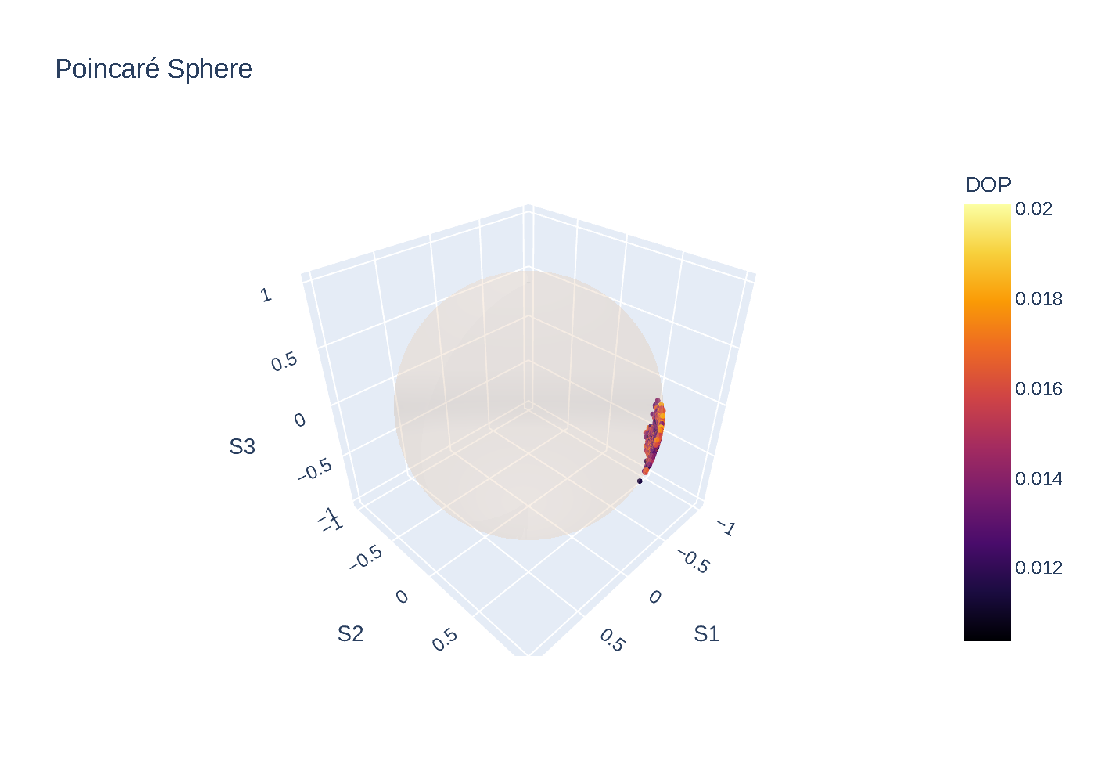
\includegraphics[width=0.9\textwidth]{Chapter 4/Figures/Distribution.pdf}
            \caption{Caption}
            \label{fig:enter-label}
        \end{figure}
        
